% !TEX root = ../thesis.tex
% !TEX spellcheck = en-US

\thispagestyle{empty}

\section{Experimental Results}
\label{sec:Experimental Results}

With the final problem definition and dataset in place a series of experiments were conducted to evaluate the performance of the different approaches explained in Section~\ref{sec:Methods}.
This part of the thesis lays out these experiments and their results. First the research objectives will be defined and the metrics used for evaluation will be described. Next the experimental setup for each of the methods will be described and the outcomes and observations will be presented.

\subsection{Objectives and Metrics}
\label{sub:Objectives and Metrics}

The experiments had simple objectives: The goal was to evaluate each method in terms of its effectiveness using a prediction metric well-suited for this problem. Further additional considerations, especially algorithmic time and space complexity were taken into account by comparing methods with regards to their runtime and need for computational resources.

\glsreset{MCC} % reset MCC in case the reader has forgotten

As a metric for predictive performance \gls{MCC} was chosen. This metric is used relatively rarely used in the machine learning literature as opposed to e.g.\ the F1 score that is common in the \gls{IR} literature where ignoring True Negatives can be tolerated. As an example we do not generally care if a search engine predicts correctly all the billions of website we don't want to see for a search query as long as it retrieves enough relevant ones.
However, with the dataset at hand a metric was needed that measures prediction reliably and without bias even in case of a strongly skewed distribution of labels. Stratified sampling from the dataset to achieve a balanced distribution was not an option since the dataset was too small. Thus \gls{MCC} was chosen which fulfills these criteria as Section~\ref{sub:Evaluation Metrics} points out and additionally is easy to interpret: It is a correlation score between -1 and 1, denoting anti-correlation and correlation respectively. In some experiments additionally further metrics were measured.

\subsection{Baseline}
\label{sub:Baseline}

In order to have a reference point for predictive performance that any method should surpass two guessing strategies were used, namely uniform and stratified guessing. Uniform guessing means sampling from a uniform distribution, commonly known as ``rolling dice'', while stratified guessing refers to an estimator that samples a label for a data point using the observed distribution of labels in the data. Both methods effectively ignore the data itself when producing labels and as such any predictive algorithm should do better.

Averaged over 1000 runs both strategies yielded an \gls{MCC} score close to zero. Accuracy by comparison was around 0.16 for uniform guessing and 0.26 for stratified guessing. These results are within our expectations and further highlight the rationale for choosing \gls{MCC} as the principal metric: \gls{MCC} is zero for uninformed predictions for either strategy whereas the accuracy in the uniform setting corresponds simply to a value of $1/k$ where $k = 6$ is the number of labels. The accuracy in the stratified setting reveals improves by taking advantage of knowledge about the skew in the label distribution. Figure~\ref{fig:guessing-conf-matrix} shows the confusion matrices for these baseline variants in absolute and normalized form, where the described properties these guessing strategies can be observed.

\begin{figure}
 % From http://localhost:8888/notebooks/thesis/experiments/vector-space-models/Vector%20Space%20Models.ipynb#Baseline:-Guessing-Strategies
    \centering
    \begin{subfigure}[b]{0.47\textwidth}
        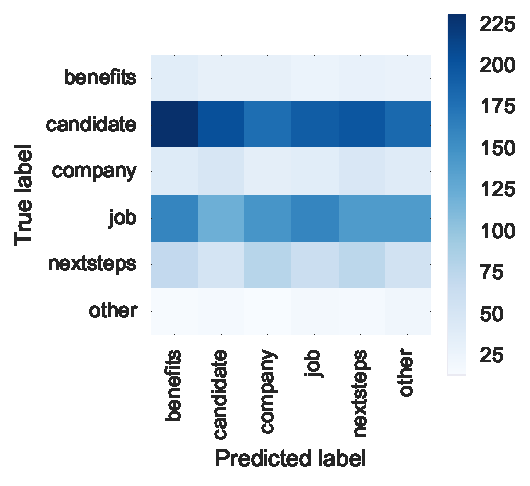
\includegraphics[width=\textwidth]{img/exp-vector-space/guessing-conf-matrix-uniform.pdf}
        \caption{Uniform guessing}
\label{fig:guessing-conf-matrix-uniform}
    \end{subfigure}
~\begin{subfigure}[b]{0.48\textwidth}
        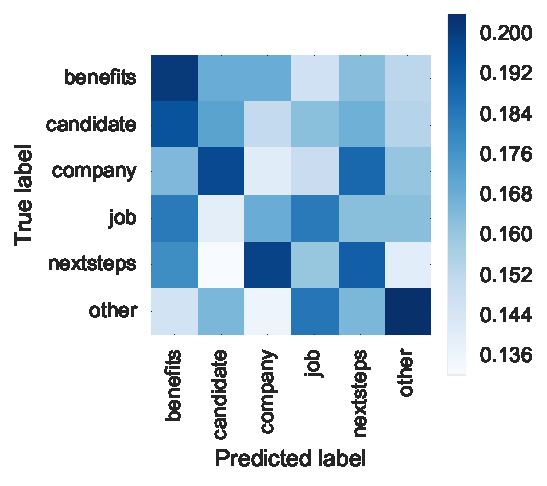
\includegraphics[width=\textwidth]{img/exp-vector-space/guessing-conf-matrix-uniform-normalized.pdf}
        \caption{Uniform guessing (normalized)}
\label{fig:guessing-conf-matrix-uniform-normalized}
    \end{subfigure}
~\begin{subfigure}[b]{0.47\textwidth}
        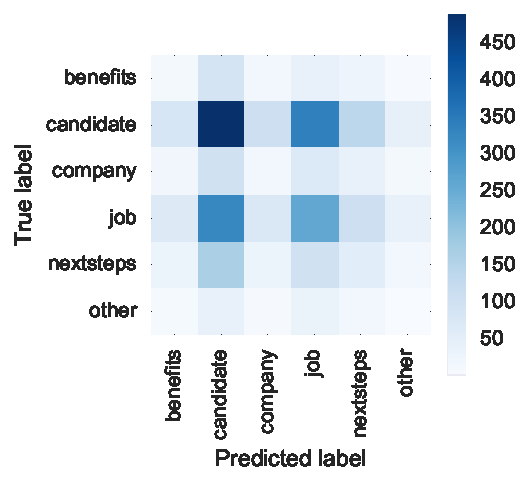
\includegraphics[width=\textwidth]{img/exp-vector-space/guessing-conf-matrix-stratified.pdf}
        \caption{Stratified guessing}
\label{fig:guessing-conf-matrix-stratified}
    \end{subfigure}
~\begin{subfigure}[b]{0.48\textwidth}
        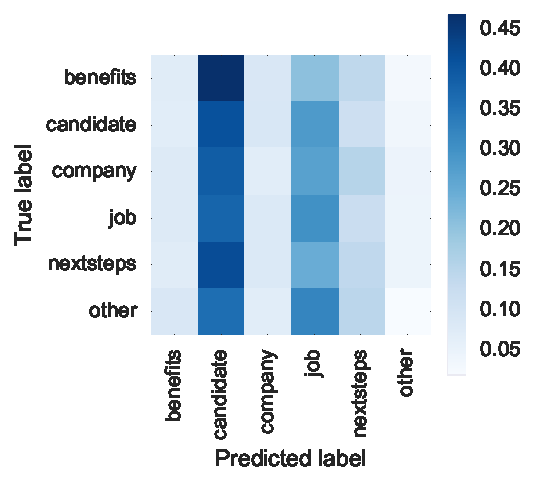
\includegraphics[width=\textwidth]{img/exp-vector-space/guessing-conf-matrix-stratified-normalized.pdf}
        \caption{Stratified guessing (normalized)}
\label{fig:guessing-stratified-normalized}
    \end{subfigure}
    \caption{Confusion matrices of uniform and stratified guessing strategies.}
\label{fig:guessing-conf-matrix}
\end{figure}

\clearpage

\subsection{Classification With Vector Space Models}
\label{sub:Classification With Vector Space Models}

A popular way to approach text classification and other tasks in natural language processing is to build a model that maps data into a vector space. Distance between data points in this space then translates to similarity between the objects (see Section~\ref{sub:Vector Space Models}).
The resulting vector representation of the data can then be fed into various learning algorithms. This section describes the experiments performed to evaluate such approaches.

First the different methods to produce such vector spaces are compared. Several methods were used to generate vectors from the data while limiting dimensionality to 300 for comparability --- a heuristically chosen value as performance for the models did not increase significantly beyond it. These vector representations were then compared in terms of performance by using them as input to the simple classification model Logistic Regression.
Second, the best performing configurations for each type of method were chosen and a set of various classification techniques were applied to them which were described previously in Section~\ref{sub:Methods For Classification With Vector Space Models}.

\subsubsection{N-gram Models}
\label{subs:N-gram Models (Experimental Results)}

The first class of language models that was investigated for the task of multi-class classification are N-gram models that were explained in Section~\ref{subs:N-gram Models (Methods)}.
N-gram models come in a variety of forms. In these experiments the most common variants were set up as hyper-parameters to the model as  listed in Table~\ref{tab:N-gram Hyper-parameters Space}.

\begin{table}[h]
  \begin{center}
  \begin{tabular}{ l l l}
    \toprule
    Hyper-Parameter & N-gram Type: Words & N-gram Type: Characters \\
    \midrule
    N-gram Range (Range) & [1,1], [1,2], [1,3], [2,3], [3,3] & [1,5], [1,10], [5,10], [5,15] \\
    Stop Words & English, None & N/A \\
    Vector Size (Size) & 10, 100, 300 & 10, 100, 300 \\
    IDF & Yes, No & Yes, No \\
    Norm & L1, L2, None & L1, L2, None \\
    Sub-linear TF & Yes, No & Yes, No \\
    \bottomrule
  \end{tabular}
  \caption{Parameter search space for word and character level N-gram models}
\label{tab:N-gram Hyper-parameters Space}
\end{center}
\end{table}

A grid search was performed to test all combinations of configurations within this hyper-parameter space. Each configuration was evaluated with regards to its \gls{MCC} score using 5-fold cross-validation on the training data with three standard classifiers: Logistic Regression and Naive Bayes and SVM.
Table~\ref{tab:Ngram Grid Search} shows the five best results of the exhaustive grid search over the hyper-parameter configurations.

\begin{table}[h]
  \begin{center}
  \begin{tabular}{ l l l l l l l l }
    \toprule
    Type & Range & Stop words & Size & IDF & Norm & Sub-linear TF & \gls{MCC} \\
    \midrule
    Word & [1,1] & None & 300 & Yes &  & Yes & 0.689 \\
    Word & [1,1] & None & 300 & Yes &  & No & 0.687 \\
    Word & [1,1] & None & 300 & No &  & Yes & 0.682 \\
    Word & [1,1] & None & 300 & No &  & No & 0.682 \\
    Word & [1,1] & None & 300 & Yes & L2 & Yes & 0.68 \\
    \midrule
    Word & [1,1] & None & 300 & No & & Yes & 0.659  \\
    Word & [1,1] & None & 300 & No & & No & 0.656 \\
    Word & [1,2] & None & 300 & No & & Yes & 0.655 \\
    Word & [1,2] & None & 300 & No & & No & 0.655 \\
    Word & [1,3] & None & 300 & No & & No & 0.65 \\
    \midrule
    Word & [1,1] & None & 300 & Yes & & Yes & 0.689 \\
    Word & [1,1] & None & 300 & Yes & & No  & 0.689 \\
    Word & [1,2] & None & 300 & Yes & & Yes & 0.677 \\
    Word & [1,2] & None & 300 & Yes & & No  & 0.677 \\
    Word & [1,3] & None & 300 & Yes & & Yes & 0.674 \\
    \bottomrule
  \end{tabular}
  \caption{Top 5 results of grid search over hyper-parameter space using 5-fold cross-validation on the training set with Logistic Regression (top), Naive Bayes (middle) and SVM (bottom).}
\label{tab:Ngram Grid Search}
\end{center}
\end{table}

The following observations can be made from the results of the grid search with regards to each of hyper-parameters:

\paragraph{Type}
\label{par:Type}
Words as the atomic unit for N-grams consistently led to better results. This can be explained by the fact that the search space of combinations of characters is significantly larger than the search space of known words, so model complexity increases exponentially.

\paragraph{Range}
\label{par:Range}
With regards to the range, i.e.\ the interval for possible $N$ in N-grams, there are slight differences to be observed between the three classifiers used, but with all three models the best performance is achieved using Unigrams. Also all of the top results across all classifiers include Unigrams in the model while some extend the range towards bigrams or trigrams.

\paragraph{Stop Words}
\label{par:Stop Words}
None of the top results of the performed grid searches used stop words. This is interesting as using stop-words to remove hand-picked, highly frequent words that do not carry much meaning is common practice.

\paragraph{Size}
\label{par:Size}
For the given settings the highest vector dimensionality of 300 achieves the best performance.

\paragraph{IDF}
\label{par:IDF}
There is no consensus between the classifiers on whether or not to weigh the N-gram frequencies by the inverse document frequency (see Section~\ref{subp:TF.IDF weighting}).

\paragraph{Norm}
\label{par:Norm}
In these experiments normalizing vectors decreased performance.
Only in the fifth best performing configuration when using Logistic Regression vectors were normalized, in this case using the L2 norm.

\paragraph{Sub-linear TF}
\label{par:Sub-linear TF}
Applying sub-linear term frequency scaling (see Section~\ref{subp:Sublinear TF scaling}) did not seem to affect the results significantly and about half of the top results were obtained using this technique.
\bigskip

Finally to the best model for each classifier with regards to \gls{MCC} validation score was chosen and trained on the whole training data and tested on the test data set to estimate the final performance. Table~\ref{tab:Ngram Grid Search Scores} shows the scores of each classifier using these best N-gram models. It is evident that here logistic regression performs best, achieving the highest \gls{MCC} score as well as good accuracy.

\begin{table}
  \begin{center}
  \begin{tabular}{ r | *2l | *2l }
    \toprule
     & \multicolumn{2}{c|}{Training} & \multicolumn{2}{c}{Test}\\
    Classifier & Accuracy & MCC & Accuracy & MCC \\
    \midrule
    Logistic Regression & 0.824 & 0.761 & 0.787 & 0.708 \\
    Naive Bayes         & 0.769 & 0.681 & 0.767 & 0.677 \\
    SVM                 & 0.835 & 0.681 & 0.786 & 0.700 \\
    \bottomrule
  \end{tabular}
  \caption{Performance of each best N-gram model with Logistic Regression and Naive Bayes on the test data.}
\label{tab:Ngram Grid Search Scores}
\end{center}
\end{table}

\begin{figure}
    \centering
    \begin{subfigure}[b]{0.3595\textwidth}
        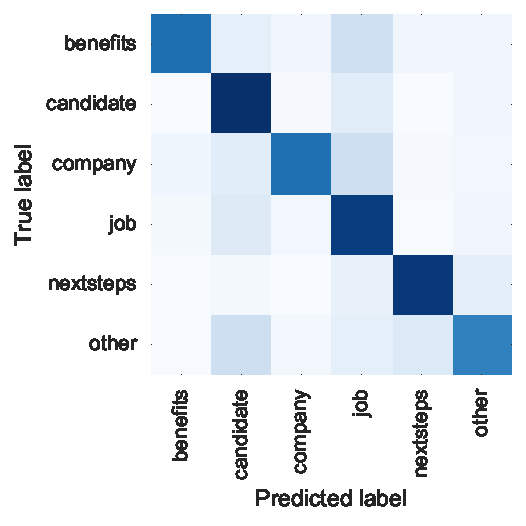
\includegraphics[width=\textwidth]{img/exp-vector-space/ngram-conf-matrix-logreg-normalized.pdf}
        \caption{Logistic Regression}
\label{fig:ngram-conf-matrix-logreg-normalized}
    \end{subfigure}
    \begin{subfigure}[b]{0.267\textwidth}
        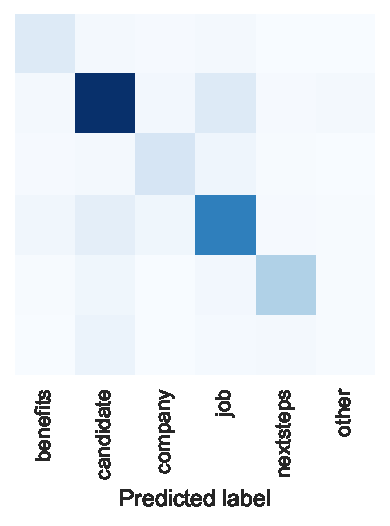
\includegraphics[width=\textwidth]{img/exp-vector-space/ngram-conf-matrix-naivebayes-normalized.pdf}
        \caption{Naive Bayes}
\label{fig:ngram-conf-matrix-naivebayes-normalized}
    \end{subfigure}
    \begin{subfigure}[b]{0.35\textwidth}
        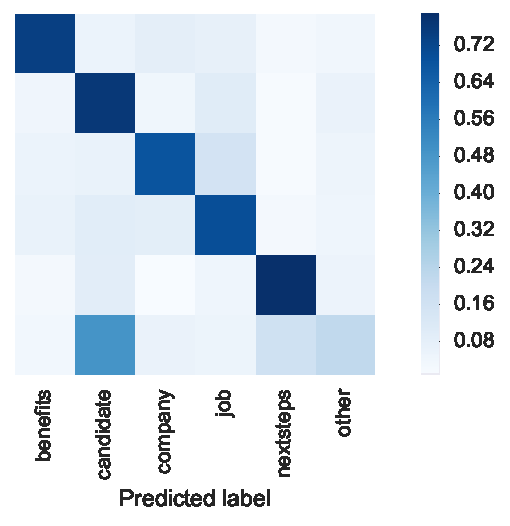
\includegraphics[width=\textwidth]{img/exp-vector-space/ngram-conf-matrix-svm-normalized.pdf}
        \caption{SVM}
\label{fig:ngram-conf-matrix-svm-normalized}
    \end{subfigure}
    \caption{Normalized confusion matrices all three classifiers using the best N-gram model found via cross-validated grid search. Both Naive Bayes as well as SVM show label bias towards the prevalent class \emph{candidate}.}
\label{fig:ngram-conf-matrix}
\end{figure}

To understand the mapping of the data in the resulting vector space visualizations were produced using \gls{PCA} and \gls{t-SNE}. The results for best-performing N-gram model can be seen in Figure~\ref{fig:ngram pca and tsne}. Especially the \gls{PCA} visualization shows that a high percentage of the data for each class can be separated from other classes even with a linear model.

\begin{figure}[h]
    \centering
    \begin{subfigure}[b]{0.48\textwidth}
      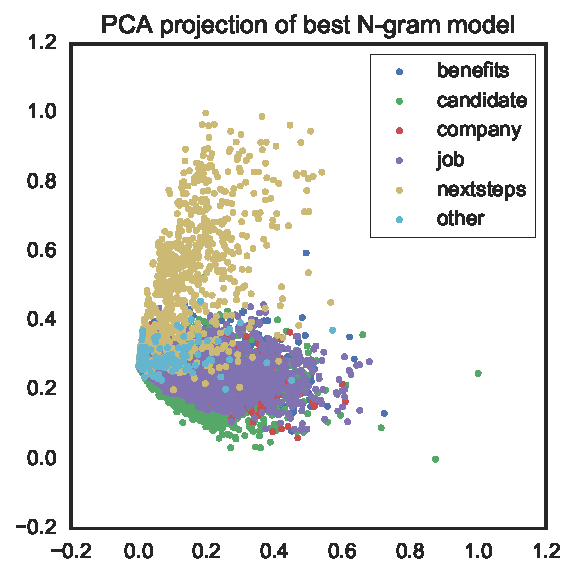
\includegraphics[width=\textwidth]{img/exp-vector-space/ngram-pca.pdf}
      \caption{PCA projection}
\label{fig:ngram-pca}
    \end{subfigure}
~
    %add desired spacing between images, e. g. ~, \quad, \qquad, \hfill etc.
    %(or a blank line to force the subfigure onto a new line)
    \begin{subfigure}[b]{0.48\textwidth}
      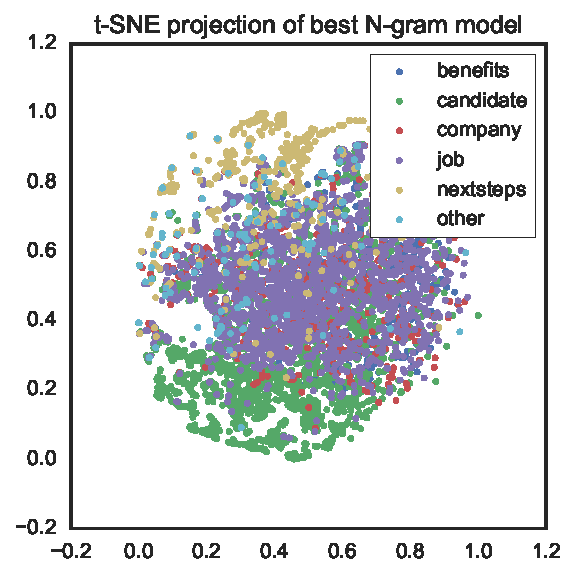
\includegraphics[width=\textwidth]{img/exp-vector-space/ngram-tsne.pdf}
      \caption{t-SNE projection}
\label{fig:ngram-tsne}
    \end{subfigure}
    \caption{Document vectors produced by the best N-gram model (optimized w.r.t. Logistic Regression) projected onto the first 2 principal components (left) and project using t-SNE projection.}
\label{fig:ngram pca and tsne}
\end{figure}

\subsubsection{Bag-of-Means: An Averaged Word2Vec Model}
\label{subs:Bag-of-Means: An Averaged Word2Vec Model}

Next a Bag-of-Means model as described in Section~\ref{subp:Bag-of-Means} was evaluated with the same set of classifiers. The model was evaluated on the same test and training data split as used for the N-gram model above. The results are shown in Table~\ref{tab:Bag-Of-Means Results}.

\begin{table}[h]
  \begin{center}
  \begin{tabular}{ r | *2l | *2l }
    \toprule
     & \multicolumn{2}{c|}{Training} & \multicolumn{2}{|c}{Test}\\
    Classifier & Accuracy & MCC & Accuracy & MCC \\
    \midrule
    Logistic Regression & 0.797 & 0.722 & 0.784 & 0.702 \\
    Naive Bayes         & 0.337 & 0.271 & 0.320 & 0.251 \\
    SVM                 & 0.545 & 0.356 & 0.562 & 0.379 \\
    \bottomrule
  \end{tabular}
  \caption{Performance base classifiers using the Bag-of-Means model}
\label{tab:Bag-Of-Means Results}
\end{center}
\end{table}

As a basis, pre-trained word vectors from the Google News dataset\footnote{The dataset contains contains 300-dimensional vectors for 3 million words and phrases. The phrases were obtained using a simple data-driven approach described in~\cite{Mikolov:2013ab}. The dataset can be obtained on the following website: \url{https://code.google.com/archive/p/word2vec/}} were extracted for the words that occur in the dataset.
Then for each sentence in the data a sentence vector was obtained by taking the arithmetic mean over the vectors for all words in the sentence. Labels were again predicted using Logistic Regression, Naive Bayes and SVM.
We can see that the model performs well using Logistic Regression and it is almost on par with the best N-gram model. On the other hand the variance in results between the classifiers is drastic, and Naive Bayes' score is 0.451 lower that Logistic Regression in absolute terms. The confusion matrices in Figure~\ref{fig:bom-conf-matrix} reveal strong label bias in the case of Naive Bayes and SVM.

\begin{figure}[h]
    \centering
    \begin{subfigure}[b]{0.365\textwidth}
        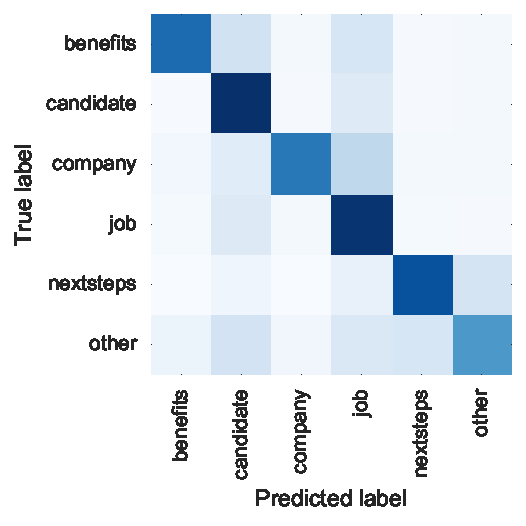
\includegraphics[width=\textwidth]{img/exp-vector-space/bom-conf-matrix-logreg-normalized.pdf}
        \caption{Logistic Regression}
\label{fig:bom-conf-matrix-logreg-normalized}
    \end{subfigure}
    \begin{subfigure}[b]{0.27\textwidth}
        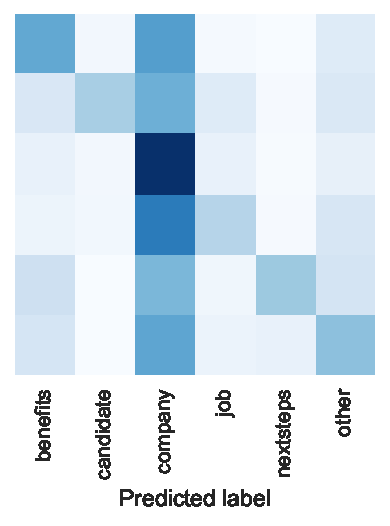
\includegraphics[width=\textwidth]{img/exp-vector-space/bom-conf-matrix-naivebayes-normalized.pdf}
        \caption{Naive Bayes}
\label{fig:bom-conf-matrix-naivebayes-normalized}
    \end{subfigure}
    \begin{subfigure}[b]{0.345\textwidth}
        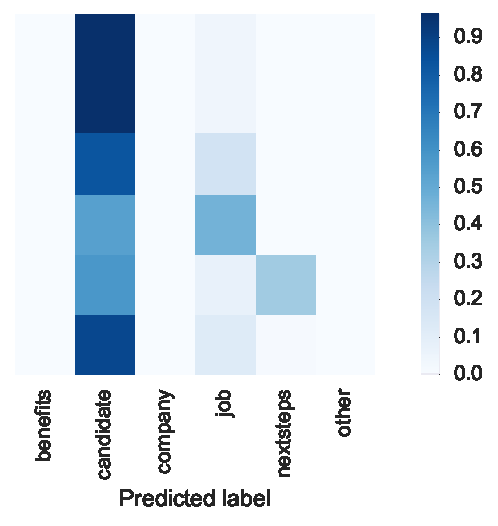
\includegraphics[width=\textwidth]{img/exp-vector-space/bom-conf-matrix-svm-normalized.pdf}
        \caption{SVM}
\label{fig:bom-conf-matrix-svm-normalized}
    \end{subfigure}
    \caption{Normalized confusion matrices of all three classifiers using the Bag-of-Means model.}
\label{fig:bom-conf-matrix}
\end{figure}

Figure~\ref{fig:bom} again visualizes a projection of the vectors into a 2 dimensional space, showing that labels tend to cluster.

\begin{figure}[h!]
    \centering
    \begin{subfigure}[b]{0.48\textwidth}
      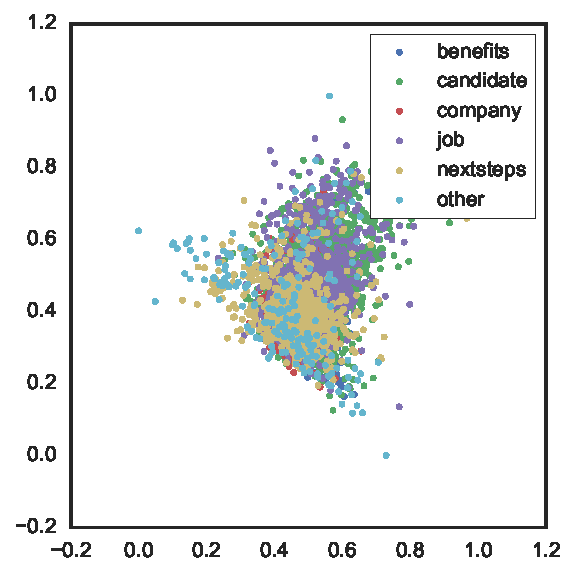
\includegraphics[width=\textwidth]{img/exp-vector-space/bom-pca.pdf}
      \caption{PCA projection}
\label{fig:bom-pca}
    \end{subfigure}
~
    %add desired spacing between images, e. g. ~, \quad, \qquad, \hfill etc.
    %(or a blank line to force the subfigure onto a new line)
    \begin{subfigure}[b]{0.48\textwidth}
      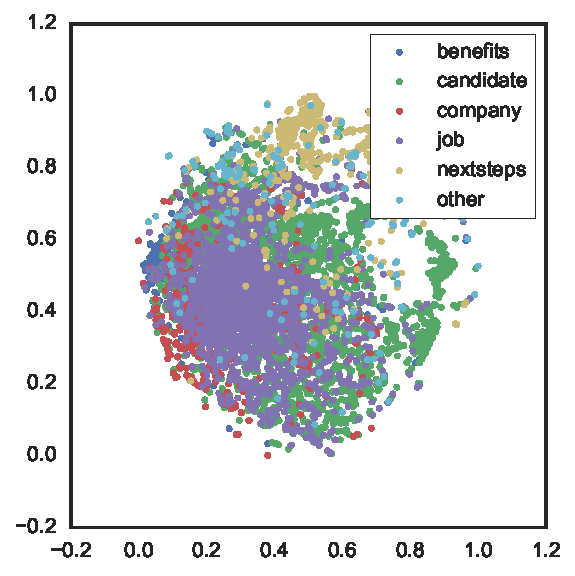
\includegraphics[width=\textwidth]{img/exp-vector-space/bom-tsne.pdf}
      \caption{t-SNE projection}
\label{fig:bom-tsne}
    \end{subfigure}
    \caption{Document vectors produced by Bag-of-Means model (optimized w.r.t. Logistic Regression) projected onto the first 2 principal components (left) and projected using t-SNE projection. It is clear that even though the vectors are simply obtained by averaging they do indeed produce somewhat seperable manifolds.}
\label{fig:bom}
\end{figure}

\subsubsection{Paragraph Vectors using Distributed Representations}
\label{subs:Paragraph Vectors using Distributed Representations}

\todo{Doc2Vec model is evaluated in 2 ways (normal and trained on inferred vectors)}

Next a vector space model was build using the approach proposed by~\cite{Le:2014aa} and described in more detail in Section~\ref{par:Distributed representations for documents}. Again there are several hyper-parameters to this model that are described in Section~\ref{subs:Language Models using Distributed Representations} and turn out to have a huge influence on its performance as the results below indicate. As this model is computationally quite expensive a grid search as for the N-gram model above was infeasible. Thus the effect of the hyper-parameters was studied by just varying them one at a time while keeping the others fixed, using a Logistic Regression classifier with 5-fold cross-validation.


%%%%%%%%%%%


The next sections will briefly outline the results of these tests:\footnote{All tables in this section will use the following abbreviations: \emph{type}: Model Type, i.e. PV-DM vs. PV-DBOW; \emph{size}: Vector Size; \emph{window}: Window Size; \emph{negative}: Negative Sampling value $k$; \emph{hs}: Hierarchical Softmax used; \emph{sample}: Frequent word sub-sampling threshold; \emph{MCC}: Matthews Correlation Coefficient}

\paragraph{Vector Size}
As was to expect the vector size of the model correlates with the performance. Again the highest chosen dimensionality was 300 which yielded the best results with a Matthews Correlation Coefficient of 0.53, however the difference to a 100-dimensional model was marginal with 1\% absolute improvement. Surprisingly even a 10-dimensional vector space model is capable of achieving almost best results with a difference of only 2\% to the 300-dimensional model. Even a 2-dimensional model could achieve a MCC score of 14\%.

\begin{table}[h]
  \begin{center}
    \begin{tabular}{ c | *2c | *2c }
      \toprule
       & \multicolumn{2}{c|}{MCC Training} & \multicolumn{2}{|c}{MCC Test}\\
      Vector Size & Trained & Inferred & Trained & Inferred \\
      \midrule
      2   & 0.302 & 0.255 & 0.173 & 0.251 \\
      10  & 0.457 & 0.417 & 0.296 & \textbf{0.405} \\
      100 & 0.535 & 0.358 & 0.341 & 0.384 \\
      300 & 0.575 & 0.363 & 0.347 & 0.393 \\
      \bottomrule
    \end{tabular}
  \caption{Matthews Correlation Coefficient with varying vector size.}
\label{tab:Paragraph Vector Parameter Results Size}
\end{center}
\end{table}

\begin{figure}[h!]
    \centering
    \begin{subfigure}[b]{0.49\textwidth}
      \includegraphics[width=\textwidth]{img/exp-vector-space/doc2vec_vector_size_2}
      \caption{Vector Size: 2}
\label{fig:doc2vec_vector_size_2}
    \end{subfigure}
    \begin{subfigure}[b]{0.49\textwidth}
      \includegraphics[width=\textwidth]{img/exp-vector-space/doc2vec_vector_size_10}
      \caption{Vector Size: 10}
\label{fig:doc2vec_vector_size_10}
    \end{subfigure}
    \begin{subfigure}[b]{0.49\textwidth}
      \includegraphics[width=\textwidth]{img/exp-vector-space/doc2vec_vector_size_100}
      \caption{Vector Size: 100}
\label{fig:doc2vec_vector_size_100}
  \end{subfigure}
  \begin{subfigure}[b]{0.49\textwidth}
    \includegraphics[width=\textwidth]{img/exp-vector-space/doc2vec_vector_size_300}
    \caption{Vector Size: 300}
\label{fig:doc2vec_vector_size_300}
  \end{subfigure}
\caption{test}
\label{fig:doc2vec_vector_size}
\end{figure}

\paragraph{Frequent Word Sub-Sampling}
Frequent word sub-sampling can boost performance quite much, but again choosing the right value for this hyper-parameter is key. The training behavior with different sampling thresholds differs quite much. Figure~\ref{fig:doc2vec-param-sample} shows the training with different values with 100 passes over the dataset. A good value seems to be $10^{-5}$ which achieves an MCC score of 0.697 and is on-par with the best N-gram model. Interestingly not using sub-sampling in this setup seemed to be overfitting as the score decreases quite drastically with more training passes. A similar effect is observed with a higher threshold of $10^{-4}$ but much less strong. Choosing a lower threshold of $10^{-6}$ leads to very poor performance with an MCC score of only 0.07.

\begin{table}[h]
  \begin{center}
    \begin{tabular}{ c | *2c | *2c }
      \toprule
       & \multicolumn{2}{c|}{MCC Training} & \multicolumn{2}{|c}{MCC Test}\\
      Sub-sampling threshold & Trained & Inferred & Trained & Inferred \\
      \midrule
      No sub-sampling & 0.536 & 0.363 & 0.336 & 0.384 \\
      1e-4 & 0.627 & 0.377 & 0.315 & \textbf{0.397} \\
      1e-5 & 0.599 & 0.250 & 0.173 & 0.247 \\
      1e-6 & 0.431 & 0.147 & 0.106 & 0.129 \\
    \bottomrule
  \end{tabular}
  \caption{Matthews Correlation Coefficient with varying frequent word sub-sampling threshold.}
\label{tab:Paragraph Vector Parameter Results Sample}
\end{center}
\end{table}

\begin{figure}[h!]
    \centering
    \begin{subfigure}[b]{0.49\textwidth}
      \includegraphics[width=\textwidth]{img/exp-vector-space/doc2vec_sample_0}
      \caption{No Sub-Sampling}
\label{fig:doc2vec_sample_0}
    \end{subfigure}
    \begin{subfigure}[b]{0.49\textwidth}
      \includegraphics[width=\textwidth]{img/exp-vector-space/doc2vec_sample_1e-4}
    \caption{Sub-Sampling Threshold: 1e-4}
\label{fig:doc2vec_vector_size_1e-4}
    \end{subfigure}
    \begin{subfigure}[b]{0.49\textwidth}
      \includegraphics[width=\textwidth]{img/exp-vector-space/doc2vec_sample_1e-5}
      \caption{Sub-Sampling Threshold: 1e-5}
\label{fig:doc2vec_vector_size_1e-5}
  \end{subfigure}
  \begin{subfigure}[b]{0.49\textwidth}
    \includegraphics[width=\textwidth]{img/exp-vector-space/doc2vec_sample_1e-6}
    \caption{Sub-Sampling Threshold: 1e-6}
\label{fig:doc2vec_sample_1e-6}
  \end{subfigure}
\caption{test}
\label{fig:doc2vec_sample}
\end{figure}

\paragraph{Hierarchical Softmax}
Using hierarchical softmax increased the performance, leading to a 12\% absolute difference in terms of MCC score. This result is counter-intuitive as using the hierarchical softmax should as an approximation be less performant. However it might simply mitigate overfitting of the model.

\begin{table}[h]
  \begin{center}
    \begin{tabular}{ c | *2c | *2c }
      \toprule
       & \multicolumn{2}{c|}{MCC Training} & \multicolumn{2}{|c}{MCC Test}\\
      Hierarchical Softmax & Trained & Inferred & Trained & Inferred \\
      \midrule
      Not used & 0.364 & 0.195 & 0.201 & 0.236 \\
      Used     & 0.534 & 0.365 & 0.340 & \textbf{0.387} \\
    \bottomrule
  \end{tabular}
  \caption{Matthews Correlation Coefficient with and without using hierarchical softmax.}
\label{tab:Paragraph Vector Parameter Results Hierarchical Softmax}
\end{center}
\end{table}

\begin{figure}[h!]
    \centering
    \begin{subfigure}[b]{0.49\textwidth}
      \includegraphics[width=\textwidth]{img/exp-vector-space/doc2vec_hs_0}
      \caption{Without Hierarchical Softmax}
\label{fig:doc2vec_hs_0}
    \end{subfigure}
    \begin{subfigure}[b]{0.49\textwidth}
      \includegraphics[width=\textwidth]{img/exp-vector-space/doc2vec_hs_1}
    \caption{With Hierarchical Softmax}
\label{fig:doc2vec_hs_1}
    \end{subfigure}
\caption{test}
\label{fig:doc2vec_hs}
\end{figure}

\paragraph{Negative Sampling}
Negative Sampling generally increased the performance of the model and smaller values actually worked best out of the tested settings from 0 to 6. Choosing the number of negative samples to be 2 resulted in the best performance, but the absolute difference in performance was only about 6\% of achieved MMC score.

\begin{table}[h]
  \begin{center}
    \begin{tabular}{ c | *2c | *2c }
      \toprule
       & \multicolumn{2}{c|}{MCC Training} & \multicolumn{2}{|c}{MCC Test}\\
      Negative Sampling Value & Trained & Inferred & Trained & Inferred \\
      \midrule
      0 & 0.581 & 0.221 & 0.332 & 0.343 \\
      2 & 0.555 & 0.338 & 0.363 & \textbf{0.399} \\
      4 & 0.517 & 0.336 & 0.350 & 0.378 \\
      6 & 0.489 & 0.317 & 0.338 & 0.363 \\
    \bottomrule
  \end{tabular}
  \caption{Matthews Correlation Coefficient with varying negative sampling value.}
\label{tab:Paragraph Vector Parameter Results Negative Sampling}
\end{center}

\end{table}

\begin{figure}[h!]
    \centering
    \begin{subfigure}[b]{0.49\textwidth}
      \includegraphics[width=\textwidth]{img/exp-vector-space/doc2vec_negative_0}
      \caption{Negative Sampling Value: 2}
\label{fig:doc2vec_negative_0}
    \end{subfigure}
    \begin{subfigure}[b]{0.49\textwidth}
      \includegraphics[width=\textwidth]{img/exp-vector-space/doc2vec_negative_2}
    \caption{Negative Sampling Value: 2}
\label{fig:doc2vec_vector_size_2}
    \end{subfigure}
    \begin{subfigure}[b]{0.49\textwidth}
      \includegraphics[width=\textwidth]{img/exp-vector-space/doc2vec_negative_4}
      \caption{Negative Sampling Value: 4}
\label{fig:doc2vec_vector_size_4}
  \end{subfigure}
  \begin{subfigure}[b]{0.49\textwidth}
    \includegraphics[width=\textwidth]{img/exp-vector-space/doc2vec_negative_6}
    \caption{Negative Sampling Value: 6}
\label{fig:doc2vec_negative_6}
  \end{subfigure}
\caption{test}
\label{fig:doc2vec_negative}
\end{figure}

\paragraph{Window Size}
Window sizes of 5, 10 and 15 were experimented with which increase or decrease the width of context the model is trained on. Here a window size of 10 showed best results. It is safe to assume that increasing the window size much further does not lead to any improvement in the model as the correlation with the word should become weaker the farther we move away from it in a document or text.

\begin{table}[h]
  \begin{center}
    \begin{tabular}{ c | *2c | *2c }
      \toprule
       & \multicolumn{2}{c|}{MCC Training} & \multicolumn{2}{|c}{MCC Test}\\
      Window size & Trained & Inferred & Trained & Inferred \\
      \midrule
      5 & 0.534 & 0.358 & 0.380 & \textbf{0.411} \\
      10 & 0.540 & 0.347 & 0.366 & 0.393 \\
      15 & 0.536 & 0.317 & 0.339 & 0.373 \\
    \bottomrule
    \end{tabular}
  \caption{Matthews Correlation Coefficient with varying window size.}
\label{tab:Paragraph Vector Parameter Results Window Size}
\end{center}
\end{table}

\begin{figure}[h!]
    \centering
    \begin{subfigure}[b]{0.49\textwidth}
      \includegraphics[width=\textwidth]{img/exp-vector-space/doc2vec_window_5}
      \caption{Window Size: 5}
\label{fig:doc2vec_window_5}
    \end{subfigure}
    \begin{subfigure}[b]{0.49\textwidth}
      \includegraphics[width=\textwidth]{img/exp-vector-space/doc2vec_window_10}
    \caption{Window Size: 10}
\label{fig:doc2vec_window_10}
    \end{subfigure}
    \begin{subfigure}[b]{0.49\textwidth}
      \includegraphics[width=\textwidth]{img/exp-vector-space/doc2vec_window_15}
      \caption{Window Size: 15}
\label{fig:doc2vec_window_15}
  \end{subfigure}
\caption{test}
\label{fig:window}
\end{figure}


\paragraph{PV-DBOW versus PM-DV}
Both models for paragraph vectors proposed in~\cite{Le:2014aa} were tried, namely Distributed Bag of Words version of Paragraph Vector (PV-DBOW) and Distributed Memory version of Paragraph Vector (PV-DM). In these tests the DBOW model achieves significantly better results with an MCC that is 14\% than the PV-DM model in absolute terms. This is in contrast with the results in the aforementioned paper, where the authors state that \textquote{PV-DM is consistently better than PV-DBOW.}~\cite{Le:2014aa}.

\begin{table}[h]
  \begin{center}
    \begin{tabular}{ c | *2c | *2c }
      \toprule
       & \multicolumn{2}{c|}{MCC Training} & \multicolumn{2}{|c}{MCC Test}\\
      Window size & Trained & Inferred & Trained & Inferred \\
      \midrule
      PV-BBOW & 0.627 & 0.610 & 0.544 & \textbf{0.582} \\
      PV-DM   & 0.534 & 0.365 & 0.341 & 0.391 \\
    \bottomrule
    \end{tabular}
    \caption{Matthews Correlation Coefficient using the two models proposed in~\cite{Le:2014aa}.}
\label{tab:Paragraph Vector Parameter Results PV-DBOW versus PM-DV}
\end{center}
\end{table}

\begin{figure}[h!]
    \centering
    \begin{subfigure}[b]{0.49\textwidth}
      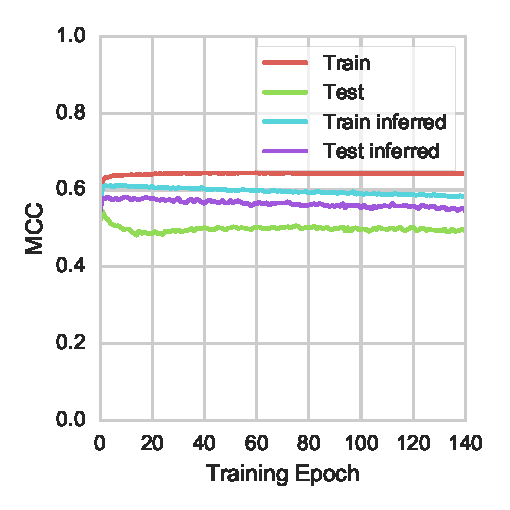
\includegraphics[width=\textwidth]{img/exp-vector-space/doc2vec_dm_0}
      \caption{PV-DBOW Model}
\label{fig:doc2vec_dm_0}
    \end{subfigure}
    \begin{subfigure}[b]{0.49\textwidth}
      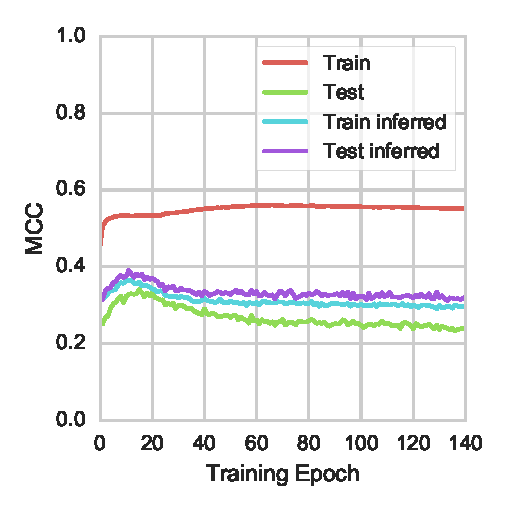
\includegraphics[width=\textwidth]{img/exp-vector-space/doc2vec_dm_1}
    \caption{PV-DM Model}
\label{fig:doc2vec_dm_1}
    \end{subfigure}
  \caption{test}
\label{fig:doc2vec_doc2vec_dm}
\end{figure}

\subsubsection{Evaluation of Classification Methods}
\label{subs:Evaluation of Classification Methods}

\paragraph{Logistic Regression}
\label{par:Logistic Regression}

\paragraph{Decision Tree}
\label{par:Decision Tree}

\paragraph{Naive Bayes}
\label{par:Naive Bayes}

\paragraph{Support Vector Machine}
\label{par:Support Vector Machine}

\paragraph{$k$ Nearest Neighbors}
\label{par:k Nearest Neighbors}

\paragraph{Random Forest}
\label{par:Random Forest}

\paragraph{Vanilla Neural Network}
\label{par:Vanilla Neural Network}

\paragraph{Deep Neural Network}
\label{par:Deep Neural Network}

\paragraph{Convolutional Neural Network}
\label{par:Convolutional Neural Network}


\subsection{Classification With Sequential Models}
\label{sub:Classification With Sequential Models}

\subsubsection{Character-based LSTM *}

\subsubsection{Stacked Character-based LSTM *}

\subsubsection{Character-based Multi-task LSTM *}
